\documentclass[11pt]{article}
\usepackage{amsmath}
\usepackage{amsthm}
\usepackage{amssymb}
\usepackage{graphicx}
\usepackage{geometry}
\usepackage{hyperref}
\usepackage[utf8]{inputenc}
\usepackage[T1]{fontenc}
\usepackage{babel}
\usepackage{tikz}
\usetikzlibrary{3d}

% Definizioni personalizzate
\newtheorem{proposition}{Proposizione}
\newtheorem{theorem}{Teorema}
\newtheorem{corollary}{Corollario}
\newtheorem{lemma}{Lemma}
\newtheorem{definition}{Definizione}
\newcommand{\oss}{\textit{Osservazione: }}
\newcommand{\R}{\mathbb R}

\begin{document}

\title{Decomposizione Matriciale SVD \\ (Singular Value Decomposition)}
\author{Federico Riva\\Ingegneria Matematica\\Politecnico di Milano}
\date{Relatore: Professor Marco Verani}

\maketitle
\newpage
\tableofcontents
\newpage
\section{Introduzione}
La decomposizione SVD è una fattorizzazione che consente di rappresentare una matrice come il prodotto di tre matrici ciascuna con caratteristiche specifiche. Le applicazioni di questo metodo possono essere ritrovate in una vasta gamma di campi tra cui l'analisi dei dati, il machine learning e l'elaborazione delle immagini.


\section{Definizione}
Sia $A\in\mathbb{R}^{m\times n}$, oppure equivalentemente $A\in\mathbb{C}^{m\times n}$, allora la decomposizione SVD della una matrice nel caso $m>n$ è definita come:

\[
A = U \Sigma V^T
\]
\[
\begin{bmatrix}
a_{11} & a_{12} & \cdots & a_{1n} \\
a_{21} & a_{22} & \cdots & a_{2n} \\
\vdots & \vdots & \ddots & \vdots \\
a_{m1} & a_{m2} & \cdots & a_{mn}
\end{bmatrix} = \mathbf{[u_1 \, u_2 \, \dots \, u_m]} \begin{bmatrix}
\sigma_1 & 0 & \cdots & 0 \\
0 & \sigma_2 & \cdots & 0 \\
\vdots & \vdots & \ddots & \vdots \\
0 & 0 & \cdots & \sigma_r \\
0 & 0 & \cdots & 0 \\
\vdots & \vdots & \ddots & \vdots \\
0 & 0 & \cdots & 0
\end{bmatrix} \mathbf{[v_1 \, v_2 \, \dots \, v_n]}^T
\]
Mentre per $m<n$:
\[
\begin{bmatrix}
a_{11} & a_{12} & \cdots & a_{1n} \\
a_{21} & a_{22} & \cdots & a_{2n} \\
\vdots & \vdots & \ddots & \vdots \\
a_{m1} & a_{m2} & \cdots & a_{mn}
\end{bmatrix} = \mathbf{[u_1 \, u_2 \, \dots \, u_m]}
\begin{bmatrix}
\sigma_1 & 0 & \cdots & 0 & 0 & \cdots & 0 \\
0 & \sigma_2 & \cdots & 0 & 0 & \cdots & 0 \\
\vdots & \vdots & \ddots & \vdots & \vdots & \ddots & \vdots \\
0 & 0 & \cdots & \sigma_r & 0 & \cdots & 0
\end{bmatrix} \mathbf{[v_1 \, v_2 \, \dots \, v_n]}^T
\]
Dove:
\begin{itemize}
    \item $U\in\mathbb{R}^{m\times m}$ è una matrice ortogonale contenente i vettori singolari sinistri di $A$,
    \item $\Sigma\in\mathbb{R}^{m\times n}$ è una matrice diagonale contenente i valori singolari di $A$ ordinati in modo decrescente,
    \item $V\in\mathbb{R}^{n\times n}$ è una matrice ortogonale contenente i vettori singolari destri di $A$.
\end{itemize}

\begin{definition}
    \textbf{Matrice Ortogonale}\\ Una matrice quadrata $Q\in\mathbb{R}^{n \times n}$ si dice ortogonale se $Q^TQ=I$.
\end{definition}
\begin{definition}
    \textbf{Matrice Simmetrica}\\ Una matrice quadrata $Q\in\mathbb{R}^{n \times n}$ si dice simmetrica se $Q^T=Q$.
\end{definition}
\begin{definition}
    \textbf{Forma Quadratica}\\ Si definisce forma quadratica un polinomio di secondo grado in $n$ variabili $p: \mathbb{R}^n \rightarrow \mathbb{R}$ t.c.
    \[
    p(x)=p(x_1,\dots,x_n)=\sum_{1 \leq i,j \leq n}a_{ij}x_ix_j=a_{11}x_1^2+a_{12}x_1x_2 + \dots + a_{nn-1}x_nx_{n-1}+a_{nn}x_n^2=\mathbf{x}^TA\mathbf{x}
    \]
    dove $\mathbf{x} = (x_1, \dots, x_n)$ e $A$ è una matrice simmetrica di dimensione $n \times n$.
\end{definition}

\begin{proposition}\label{prop 1}
\textbf{}\\
\textit{Hp:} Data una qualsiasi $M\in\mathbb{R}^{m \times n}$\\
\textit{Ts:} $D=M^TM$ e $S=MM^T$ sono  matrici simmetriche e definite positive.
\end{proposition}
\begin{proof}
1) Vogliamo dimostrare che $D=D^T$. Segue quindi dalle proprietà di trasposizione del prodotto di due matrici: $D^T=(M^TM)^T=MM^T=D$. Si dimostra in maniera analoga il risultato per $S$.\\
2) Per dimostrare la semipositività della matrice $A^TA$ dal momento che è una matrice quadrata possiamo studiare il segno della forma quadratica associata. Se quest'ultima sarà positiva allora lo saranno anche tutti gli autovalori.\\
$$ \forall \mathbf{x}\neq 0: \mathbf{x} \in \R^n$$ $$\mathbf{x}^TA^TA\mathbf{x}=(A\mathbf{x})^T(A\mathbf{x})= \|A\mathbf{x}\|^2\geq 0$$
\end{proof}
\noindent
\textit{Osservazione}: Gli autovalori che otterremo dalle due matrici saranno $\geq$ 0 e potremo quindi calcolarne la radice quadrata.
\begin{proposition}\label{prop 2}
\textbf{}\\
\textit{Hp:} Sia $A \in \R^{m \times n}$\\
\textit{Ts:} $A^TA$ e $AA^t$ hanno gli stessi autovalori non nulli.
\end{proposition}
\begin{proof}
Ipotizziamo che la coppia autovalor' autovettore $(\mathbf{x},\lambda)$ sia associata alla matrice $A^TA$. Possiamo quindi scrivere $$A^TA\mathbf{x}=\lambda\mathbf{x}$$ e moltiplicando ambo i membri per $A$ otteniamo$$AA^TA\mathbf{x}=\lambda A\mathbf{x}$$
Ma allora definendo $\mathbf{y}=A\mathbf{x}$ possiamo riscrivere $$AA^T\mathbf{y}=\lambda \mathbf{y}$$
Il che conclude la dimostrazione poichè prova che  $\lambda$ è un autovalore anche della matrice $AA^T$
\end{proof}

\begin{theorem}\label{teo spetr}
\textbf{Teorema Spettrale}\\
\textit{Hp:} Data $Q\in\mathbb{R}^{n\times n}$ una matrice simmetrica\\
\textit{Ts:} È ortognalmente digonalizzabile $Q=U^{-1}DU=U^TDU$
\end{theorem}
\noindent
Prendendo in cosiderazione le \textbf{Proposizioni \autoref{prop 1}}, \textbf{\autoref{prop 2}} ed il \textbf{Teorema \ref{teo spetr}} possiamo ossservare che data una qualsiasi matrice $A$ è possibile costruire a partire da essa due matrici simmetriche ortgonalmente diagonalizzabili. Possiamo quindi fornire le seguenti definizioni.
\begin{definition}
	\textbf{Vettori Singolari di sinistra}\\ I vettori singolari di sinstra di $A$ sono gli autovettori $\mathbf{u_1, \dots ,u_m}$ di $AA^T=U^TD_lU$ e compongono la \textit{Matrice Singolare di Sinistra} $U$.
\end{definition}
\begin{definition}
	\textbf{Vettori Singolari di destra}\\ I vettori singolari di destra di $A$ sono gli autovettori $\mathbf{v_1, \dots ,v_n}$ di $A^TA=V^TD_rV$ e compongono la \textit{Matrice Singolare di destra} $V$.
\end{definition}
\begin{definition}
	\textbf{Valori Singolari}\\ I valori singolari sono le radici quadrate degli autovalori non nulli di $A^TA$ e $A^TA$\\ $\sigma_1 \geq \dots \geq \sigma_{r=\min{n,m}} \geq 0$. Inchicheremo con $r$ il numero di valori singolari che nel caso di assenza di autovalori nulli sarà $r=\min{\{m,n\}}$.
\end{definition}

\section{Legame fra la decomposizione SVD ed il Teorema Spettrale}
Da un punto di vista intuitivo la farrotizzazion SVD può essere considerata come la generalizzaizone del concetto di diagonalizzione di una matrice quadrata; infatti se la seconda può essere applicata solamente a matrici quadrate $(n \times n)$ risuulta valida per qualsiasi tipo di matrice $(m \times n)$ senza limite alcuno sulla sua forma.\\
Se $A$ ammette la fattorizzazione SVD allora $A=U\Sigma V^T$ valgono le seguenti relazioni: $$A^TA=(U\Sigma V^T)^TU\Sigma V^T=V\Sigma^TU^TU\Sigma V^T=V\Sigma^T \Sigma V^T$$
$$ AA^T=U\Sigma V^T(U\Sigma V^T)^T=\dots=U\Sigma \Sigma^T U^T$$ 
Vale duque un risultato ancora più specifico della semplice dagonalizzazione di una matricre ovvero il Teorema Spettrale

\section{Interpretazione geometrica}
Data una matrice $A \in \R^{m \times n}$ consideriamo l'applicazione lineare ad essa associata $$A: \R^n \rightarrow \R^m$$
La fattorizzazione SVD scopone la trasformazione lineare in 3 trasformazioni geometriche rappresentate dalle 3 matici $U$,$V$ e $\Sigma$ dove le matrici ortonormali rapppresentano una rotazinone o una simmetria assiale mentre la matrice $\Sigma$ è una dilatazione di intestità $\sigma_i$ lungo la componente $\mathbf{x}_i$.Di seguito illustiamo visimaente lo specifico caso $A \in \R^{2 \times 2}$ nel caso di una circonferenza di raggio unitario che viene mappata in un'ellise.
\begin{figure}[h]
    \centering
    \includegraphics[width=0.85\textwidth,height=5.35cm]{geo.png}
    \caption{Illustrazione in $\R^2$}
    \label{fig:geo}
\end{figure}
\noindent \\
Possiamo estendere questo ragionemento ad un caso più generale considerando una sfera di raggio unitario in $\R^n$ e l'ellissoide ad essa associata da $A \in \R^{m \times n}$ in $\R^m$.\\
\begin{figure}[h]
\centering
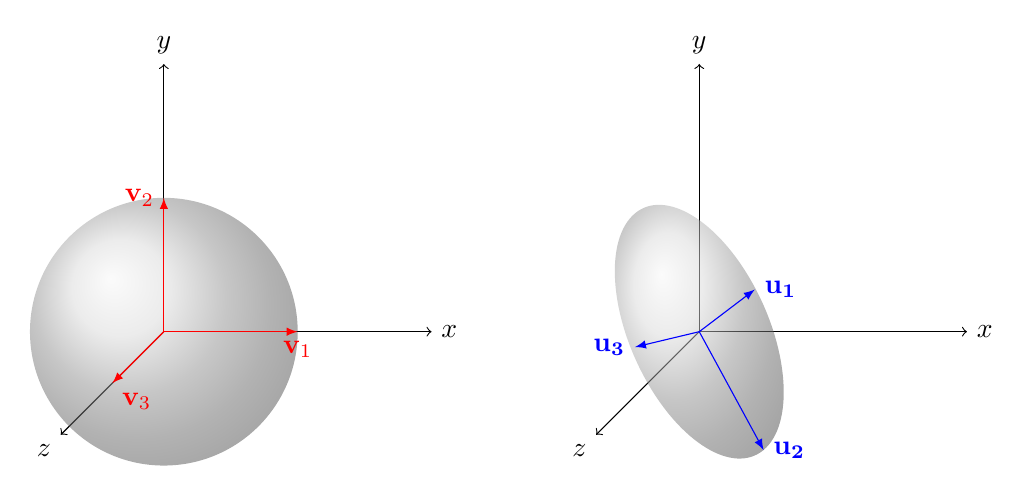
\begin{tikzpicture}[scale=1.7]
    % Prima figura - Sfera
    \begin{scope}[shift={(0,0)}]
        % Assi cartesiani
        \draw[->] (0,0,0) -- (2,0,0) node[right] {$x$};
        \draw[->] (0,0,0) -- (0,2,0) node[above] {$y$};
        \draw[->] (0,0,0) -- (0,0,2) node[below left] {$z$};
        
        % Sfera
        \shade[ball color = gray!40, opacity = 0.5] (0,0) circle (1);
        
        % Raggio della sfera
        \draw[dashed, black] (0,0) -- (1,0) node[midway, below] {};
        
        % Vettori orientati nella sfera
        \draw[-latex, red] (0,0) -- (1,0,0) node[below] {$\mathbf{v}_1$};
        \draw[-latex, red] (0,0) -- (0,1,0) node[left] {$\mathbf{v}_2$};
        \draw[-latex, red] (0,0) -- (0,0,1) node[below right] {$\mathbf{v}_3$};
    \end{scope}
    
    % Seconda figura - Ellissoide
    \begin{scope}[shift={(4,0)}]
        % Assi cartesiani
        \draw[->] (0,0,0) -- (2,0,0) node[right] {$x$};
        \draw[->] (0,0,0) -- (0,2,0) node[above] {$y$};
        \draw[->] (0,0,0) -- (0,0,2) node[below left] {$z$};
        
        % Definizione dell'ellissoide
        \def\xRadius{1} % Modificato il semiasse x
        \def\yRadius{1} % Modificato il semiasse y
        \def\zRadius{1} % Modificato il semiasse z
        
        % Disegno dell'ellissoide
        \begin{scope}[rotate around z=30,canvas is yz plane at x=0]
            \shade[ball color = gray!40, opacity = 0.5] (0,0) ellipse (\yRadius cm and \yRadius cm);
        \end{scope}
         % Calcolo della posizione della punta dell'ellisse
    \pgfmathsetmacro{\xEndPoint}{\xRadius*cos(30)}
    \pgfmathsetmacro{\yEndPoint}{\xRadius*sin(30)}
    \pgfmathsetmacro{\zEndPoint}{\zRadius}
    
    % Vettore nella punta dell'ellisse
    \draw[-latex, blue] (0,0,0) -- (0.8,0.7,1) node[right] {$\mathbf{u_1}$};
    \draw[-latex, blue] (0,0,0) -- (\xEndPoint,-\yEndPoint,\zEndPoint) node[right] {$\mathbf{u_2}$};
    \draw[-latex, blue] (0,0,0) -- (-\xEndPoint,-\yEndPoint,-\zEndPoint)node[left] {$\mathbf{u_3}$};
    \end{scope}
\end{tikzpicture}
\caption{Mappa da una sfera in $\R^n$ ad un'ellisoide in $\R^m$.}
\end{figure}
\noindent
Notiamo che le matrici $U$ e $V$ sono unitarie e le colonne di ciscuna formano una mase di vettori ortonormali. Inoltre la matrice $A$ mappa il $v_i$ elemento della base in nel vettore dilatao $\sigma_iu_i$.
\newpage
\noindent
Verifichiamolo:
\[
A = U\Sigma V^T 
\]
\[
AV = U\Sigma
\]
\[ 
[A\mathbf{v_1} \, A\mathbf{v_2} \, \dots \, A\mathbf{v_n}] = [U\mathbf{\sigma_1} \, U\mathbf{\sigma_2} \, \dots \, U\mathbf{\sigma_n}]
\]
Tenendo conto che 
\[
\mathbf{\sigma_i}=[0 \, \dots \, 0 \, \sigma_i \, 0 \, \dots \, 0]
\]
Otteniamo
$$\forall i=1,\dots,n\ A\mathbf{v_i}=\sigma_i\mathbf{u_i}
$$
Possiamo quindi scivere più in generale che:  $A\mathbf{v}=\sigma\mathbf{u}$ e $A^T\mathbf{u}=\sigma\mathbf{v}$.\\
Dal punto di vista degli spazi associati allo $Span$ delle colonne di ciascuna matrice se la matrice $A$ non ha rango massimo, $\text{Rg}(A)= r < \min{\{m,n\}}$, allora susssiste la seguente relazione:
\begin{itemize}
	\item Le prime $r$ colonne di U sono una base dello $\text{Span}(A)$;
	\item Le ultime $m-r$ colonne di U sono una base del $\text{Ker}(A^T)$;
	\item Le prime $r$ colonne di $V$ sono una base dello $\text{Span}(A^T)$;
	\item Le ultime $n-r$ colonne di $V$ sonouna base del $\text{Ker}(A)$
\end{itemize} 
\textit{Osservazione:} $\text{Span}(A)=\text{Col}(A)$ e quindi $\text{Span}(A^T)=\text{Col}(A^T)=\text{Row}(A)$.\\
La dimostrazione dell'elenco delle proprietà segue dalla \textbf{Proposizione \ref{prop gal}} unita al \textbf{Teorema \ref{teo spetr}} e alla definzione di decomposizione SVD.

\begin{theorem}\label{null}
\textbf{Teorema di Nullità più rango}\\
\textit{Hp:} Sia $A\in \R^{m \times n}$ con Rg($A$)=$r$\\
\textit{Ts:} dim Ker($A$)=$n-r$
\end{theorem}
\begin{proposition}\label{prop gal}
\textbf{}\\
\textit{Hp:} $\forall A \in \R^{m \times n}$ valogno le seguenti uguaglianze\\
\textit{Ts:} $\text{Ker}(A)=\text{Ker}(A^TA),\ \text{Col}(A^T)=\text{Col}(A^TA)$ e di conseguenza $\text{Rg}(A)=\text{Rg}(A^TA)$
\end{proposition}
\begin{proof}
Osserviamo che
$$\|A\mathbf{x}\|^2=(A\mathbf{x})^T(A\mathbf{x})=\mathbf{x}^TA^TA\mathbf{x}$$
Ne segue che, se $\mathbf{x}$ appartiene al Nucleo di $A^TA$ allora $\|A\mathbf{x}\|^2=0$ e quindi $A\mathbf{x}=0$, cioè $\mathbf{x} \in \text{Ker}(A)$. Viceversa se $ \mathbf{x} \in \text{Ker}(A)$ ripercorrendo la catena di uguaglianze a retroso $\mathbf{x} \in \text{Ker}(A^TA)$ e per arbitrarietà della scelta del vettore i due nuclei sono uguali. Dall'ugualianza dei nuclei pèr il \textbf{Teorema \ref{null}} segue l'uquaglianza dei ranghi. \\
Col($A^T$)=Row($A$) è il complemento ortogonale di Ker($A$). Ma $\text{Ker}(A)=\text{Ker}(A^TA)$ il cui complemento ortogonale è Row($A^TA$). Quindi Col($A^T$) = Row($A^TA$) ma per simmetria di $A^TA$ Row($A^TA$)=Col($A^TA$) $\Rightarrow$ Col($A$)=Col($A^TA$). 
\end{proof}

\section{Dimostrazione della decomposizione SVD e Teorema Eckart-Young}

\subsection{Dimostrazione}
Data una matrice $A \in \R^{m \times n}$ poichè $A^TA \in \R^{n \times n}$ è simmetrica e semidefinita positiva segue dal Teorema Spettrale che $\exists$ una matrice ortonormale $V \in \R^{n \times n}$ tale che $$ A^TA=V\bar{D}V^T$$ e a sua volta poichè $V^{-1}=V^T$ $$V^TA^TAV=\bar{D}= \begin{bmatrix}D & 0 \\ 0 & 0\end{bmatrix}$$
dove $D \in \R^{\ell \times \ell}$ è una matrice diagonale e positiva di dimensione con $\ell \leq \min{\{m,n\}}$ il numero di autovalori non nulli della matrice $A^TA$. 
Osserviamo che per definizione di autovalori e autovettori la $i-esima$ colonna di $V$ corrisponde all' $i-esimo$ autovalore $\bar{D}_{ii}$. Di consguenza possiamo indivuare $V_1=[\mathbf{v}_1 \, \dots \, \mathbf{v}_{\ell}] \in \R^{n \times \ell}$ e $V_2=[\mathbf{v}_{\ell+1} \, \dots \, \mathbf{v}_n] \in \R^{n \times n-\ell}$ tali che $V=[V_1 \, V_2]$ che sono rispettivamente gli autovettori associati ad autovalori non nulli e nulli. 
Possiamo quindi riscrivere l'equazione come:
$$ \begin{bmatrix} V_1^T \\ V_2^T \end{bmatrix}
A^TA \begin{bmatrix} V_1 & \!\! V_2 \end{bmatrix}
= \begin{bmatrix}  V_1^TA^TAV_1 & V_1^TA^TAV_2 \\
  V_2^TA^TAV_1 & V_2^TA^TAV_2
\end{bmatrix} = \begin{bmatrix} D & 0 \\ 0 & 0 \end{bmatrix}$$
Da cui ricaviamo le seguenti equazioni:
$$V_1^TA^TAV_1=D \ \ \text{e} \ \ V_2^TA^TAV_2=0$$ 
Siamo quindi in grado di risolvere la seconda
$$\|AV_2\|_2=0 \Rightarrow AV_2=0$$ 
Costruiamo inolte le seguenti matrici di diverse dimensioni che torneranno utili in seguito:\\
\begin{itemize}
	\item$V_1^TV_1=I_{\ell}$ dove $(\ell \times n)\times(n \times \ell)=(\ell \times \ell)$
	\item$V_2^TV_2=I_{n-\ell}$ dove $(n-\ell \ \times n)\times(n \times \ n-\ell)=(n-\ell \times n-\ell)$
	\item$[V_1 V_2][V_1 V_2]^T=V_1V_1^T+V_2V_2^T=I_n$ dove\\
 	$$(n \times \ell)\times(\ell \times n)=(n \times n) \ \text{e} \ (n \times n-\ell)\times(n-\ell \times  n)=(n \times n)$$
\end{itemize}
Definiamo ora la matrice $U_1$ come: $$U_1 = A V_1 D^{-\frac{1}{2}} \in \R^{m \times \ell}\ \lbrace(m \times \ell)=(m \times n)\times(n \times \ell)\times(\ell \times \ell)\rbrace$$ sapendo che $D^{-\frac{1}{2}}$ è ben definita poiché $D_{ii} > 0$ $\forall \ i = 1, \dots, \ell$.\\
Invertendo la relazione e sostuendo $U_1$: $$A=U_1D^{\frac{1}{2}}V_1^T=AV_1D^{-\frac12}D^{\frac12}V_1^T=AV_1V_1^T$$ e sfruttando $V_1V_1^T+V_2V_2^T=I_n$ e $AV_2=0$  otteniamo: $$A=A\left( I -V_2V_2^T \right)=A-AV_2V_2^T=A-0=A$$ il che sabilisce la veridicità dalla definizione di $U_1$ proposta.\\
Abbiamo quindi quasi dimostrato il risltato completo, non ci resta che verificare che le colonne della matrice $U_1$ formino una base ortonormale: $$ U_1^TU_1=D^{-\frac12}V_1^TA^TAV_1D^{-\frac12}=D^{-\frac12}DD^{-\frac12}=I_{\ell} \in \R^{\ell \times \ell} $$
Possiamo quindi costruire il complemento orgonale di $U_1$ ovvero $U_2=\text{Span}(\text{Col}(U_1)^\perp) \in \R^{m \times n-\ell}$ in modo che $U=[U_1 \ U_2] \in \R^{m \times m}$ sia una matrice ortogonale.\\
Per concludere aggiungiamo un numero opportune di righe e colonne nulle alla matrice $D^{\frac12} \in \R^{\ell \times \ell}$ in modo da creare: $$\Sigma=\begin{bmatrix}
  \begin{bmatrix} D^\frac{1}{2} & 0 \\ 0 & 0 \end{bmatrix} \\
  0
\end{bmatrix} \in \R^{m \times n}$$
Allora sfruttando le proprietà del prodotto matriciale fra matrici a blocchi: 
$$U\Sigma V^T= [U_1 \ U_2]\begin{bmatrix}
  \begin{bmatrix} D^\frac{1}{2} & 0 \\ 0 & 0 \end{bmatrix} \\
  0
\end{bmatrix}[V_1 \ V_2]^T= \begin{bmatrix} U_1 & U_2 \end{bmatrix}
\begin{bmatrix} D^\frac{1}{2}V_1^T \\ 0 \end{bmatrix}
= U_1 D^\frac{1}{2} V_1^T = A $$\qed

\subsection{Norme Matriciali}
Dal momento che $\R^{m \times n}$ è isomorgf a $\R^{mn}$ la norma di una matrice è equivalente alla norma di un vettore. 
\begin{definition}
	\textbf{Norma}\\ Una funzione f: $\R^{m \times n} \rightarrow \R$ è detta norma se sooddisfa le seguenti proprietà
	\begin{itemize}
		\item $f(A) \geq 0 \ \forall A\in \R^{m \times n} \ \text{e} \  f(A)=0 \iff A=0 $
		\item $f(A+B)\leq f(A)+f(B)\  \, \forall A,B \in \R^{m \times n}$ 
		\item $f(\alpha A)=|\alpha|f(A), \ \ \alpha \in \R, A \in \R^{m \times n}$
	\end{itemize}
Useremo quindi la notazione $\|A\|=f(A)$ per indicare la 'norma della matrice A'. 
\end{definition}
\noindent 
Fra le numerose norme esistenti le due più frequenti sono:
\begin{definition}
\textbf{Norma di Frobenius}\\
$$\|A\|_F=\sqrt{\sum_{i=1}^m\sum_{j=1}^n|a_{ij}|^2}$$
\end{definition}
\begin{definition}
\textbf{Norma p-esima}\\
$$ \|A\|_p = \sup_{\mathbf{x} \neq 0} \frac{\|A\mathbf{x}\|_p}{\|\mathbf{x}\|_p}=\max_{\|\mathbf{x}\|_p =1} \|A\mathbf{x}\|_p
$$
\end{definition}
\begin{definition}
\textbf{Norma $\infty$}\\
$$\|A\|_\infty = \max_{1 \leq i \leq m} \sum_{j=1}^{n} |a_{ij}|$$
\end{definition}
\begin{proposition}\label{cons norm}
\textbf{}\\
\textit{Hp:} Data una matrice ortogonale $Q \in \R^{n \times n}$\\
\textit{Ts:$\forall \mathbf{x}\in \R^n \ \|Q\mathbf{x}\|=\|\mathbf{x}\|$} 
\end{proposition}
\begin{proof} $\|Q\mathbf{x}\|^2 = (Q \mathbf{x})^T(Q \mathbf{x}) = \mathbf{x}^T Q^T Q \mathbf{x} = \mathbf{x}^TI\mathbf{x} = \mathbf{x}^T\mathbf{x} = \|\mathbf{x}\|^2$
\end{proof}
\noindent
Enunciamo ora una serie di corollari che seguono dalla dimostrazione della fattorizzazione SVD.
\begin{corollary}
\textbf{}\\
\textit{Hp:} Sia $U^TAV=\Sigma$ la decomposizione SVD della matrice $A\in \R^{m \times n}$ con $m \geq n$. \\
\textit{Ts:} $\forall i=1, \dots ,n \ A \mathbf{v}_i= \sigma_i \mathbf{u}_i \text{e} A^T \mathbf{u}_i = \sigma_i \mathbf{v}_i$  
\end{corollary}
\begin{proof}
Come abbiamo già discusso precedentemente nell'intepretazione geometrica:
\[
A = U\Sigma V^T 
\]
\[
AV = U\Sigma
\]
\[ 
[A\mathbf{v_1} \, A\mathbf{v_2} \, \dots \, A\mathbf{v_n}] = [U\mathbf{\sigma_1} \, U\mathbf{\sigma_2} \, \dots \, U\mathbf{\sigma_n}]
\]
Tenendo conto che 
\[
\mathbf{\sigma_i}=[0 \, \dots \, 0 \, \sigma_i \, 0 \, \dots \, 0]
\]
Otteniamo
$$\forall i=1,\dots,n\ A\mathbf{v_i}=\sigma_i\mathbf{u_i}
$$
Analogamente si dimostra il risultato per $A^T \mathbf{u}_i = \sigma_i \mathbf{v}_i$
\end{proof}

\begin{corollary}
\textbf{}\\
\textit{Hp:} Sia $A\in \R^{m \times n}$ con $m \geq n$ \\
\textit{Ts:} $\|A\|_2=\sigma_1 \text{e} \  \|A\|_F=\sqrt{\sigma_1^2 + \dots + \sigma_r^2}$
\end{corollary}
\begin{proof}
1) \[ \|A\|_2 = \max_{\|\mathbf{x}\|_2 =1} \|A\mathbf{x}\|_2 = \max_{\|\mathbf{x}\|_2 =1} \| U \Sigma V^T \mathbf{x} \|_2 \]
Dalla \textbf{Proposizione \ref{cons norm}} sappiamo che le due matrici ortognoali $U$ e $V$ non modificano la norma. Possiamo quindi riscrivere l'uguaglianza come $$\max_{\|\mathbf{x}\|_2 =1} \|\Sigma \mathbf{x}\|_2 $$ cioè $$\max_{\|\mathbf{x}\|_2 =1} \begin{bmatrix}
\sigma_1 & 0 & \cdots & 0 \\
0 & \sigma_2 & \cdots & 0 \\
\vdots & \vdots & \ddots & \vdots \\
0 & 0 & \cdots & \sigma_r \\
0 & 0 & \cdots & 0 \\
\vdots & \vdots & \ddots & \vdots \\
0 & 0 & \cdots & 0
\end{bmatrix} \begin{bmatrix}
x_1 \\
x_2 \\
\vdots \\
x_n
\end{bmatrix}$$ 
e poichè $\sigma_1 \geq \sigma_2 \geq \dots \geq \sigma_r \geq 0$ otteniamo il massimo per $\mathbf{x}=[1 \ 0 \dots 0]^T$ ovvero $\|A\|_2= \sigma_1$
\\2)$$\|A\|_F=\sqrt{\sum_{i=1}^m\sum_{j=1}^n|a_{ij}|^2}=\sqrt{\sum_{i=1}^m\sum_{j=1}^n|(U\Sigma V^T)_{ij}|^2}$$
scrivendo il prodotto matriciale elemento per elemento otteniamo che $$(U\Sigma V^T)_{ij} = \sum_{k=1}^{r} U_{ik} \Sigma_{kk} (V^T)_{kj}=\sum_{k=1}^{r} U_{ik} \Sigma_{kk}V_{jk}$$
$$ \|A\|_F=\sqrt{\sum_{i=1}^m\sum_{j=1}^n \sum_{k=1}^{r} U_{ik} \Sigma_{kk}V_{jk}} $$ 
Tuttavia per costruzione della matrice $\Sigma$ $$\Sigma_{kk}=\sigma_k \geq 0 \ \forall k=1,\dots,r \ \text{con} \ r\leq n=\min{\{m,n\}} \ \text{e} \ \Sigma_{ij}=0 \ \forall i=1, \dots, m \ \text{e} \ \forall j=1, \dots, n$$
Otteniamo la tesi $$\|A\|_F=\sqrt{\sigma_1^2 + \dots + \sigma_r^2}$$

\end{proof}

\begin{corollary}
\textbf{}\\
\textit{Hp:}\\
\textit{Ts:} 
\end{corollary}
\begin{proof}
\end{proof}

\begin{corollary}
\textbf{}\\
\textit{Hp:}\\
\textit{Ts:} 
\end{corollary}
\begin{proof}
\end{proof}

\begin{theorem}
\textbf{Teorema di Eckart-Young}\\
\textit{Hp:} Sia $A$ una matrice $m \times n$ di rango $r$, e sia $k \in \mathbb{N} \ \text{tale che} \ 1 \leq k \leq r$.\\
\textit{Ts:} $\forall$ matrice $B$ di rango $k$, la soluzione del problema di minimo quadrato:
\[
\min_{\text{rank}(X) = k} \|A - X\|_F^2
\]
è data dalla matrice $X$ data dalla decomposizione ai valori singolari troncata di $A$, ovvero:
\[
X = \sum_{i=1}^k \sigma_i u_i v_i^T
\]
dove $\sigma_1 \geq \sigma_2 \geq \ldots \geq \sigma_r > 0$ sono i valori singolari di $A$, e $u_i$ e $v_i$ sono rispettivamente la $i$-esima colonna di $U$ e la $i$-esima colonna di $V$ nella decomposizione ai valori singolari di $A$, ovvero $A = U \Sigma V^T$, con $U$ una matrice $m \times r$, $V$ una matrice $n \times r$, e $\Sigma$ una matrice diagonale $r \times r$ contenente i valori singolari di $A$ sulla diagonale.

\end{theorem}

\newpage
\section{Algoritmi per il Calcolo}
\section{Applicazioni Teoriche}
\subsection{Pseudoinversa di una Matrice}
\subsection{Soluzione ai Minimi Quadrati}
\section{Applicazioni Pratiche}
\subsection{PCA - Principal Component Analysis}
\subsection{Compressione Immagini}
\subsection{DMD - Dyniamic Mode Decomposition}
\subsubsection{Esempio}
\end{document}
